\documentclass[../tfg.tex]{subfiles}

\begin{document}

\section{Stack canaries}

Stack canaries are \textbf{secret values placed between local buffers and the return address}. This value is \textbf{checked} before a function returns and if the value has changed, that means that it has been overwritten and the return address may be overwritten too, possibly indicating a stack overflow attack. When that situation happens, the program automatically exits to prevent the stack overflow.
The value of the canary is \textbf{changed every time the program starts} to make it unpredictable.

This countermeasure is design to check for the \textbf{stack frame integrity}, detecting when a possible stack overflow has occurred.

\begin{figure}[H]
    \centering
    \subfile{../imgs/stack_overflow_counters/stack_canary}
    \caption{Stack canary}
    \label{fig:stack_canary}
\end{figure}

\begin{figure}[H]
    \centering
\begin{minipage}[c]{0.427\linewidth}
    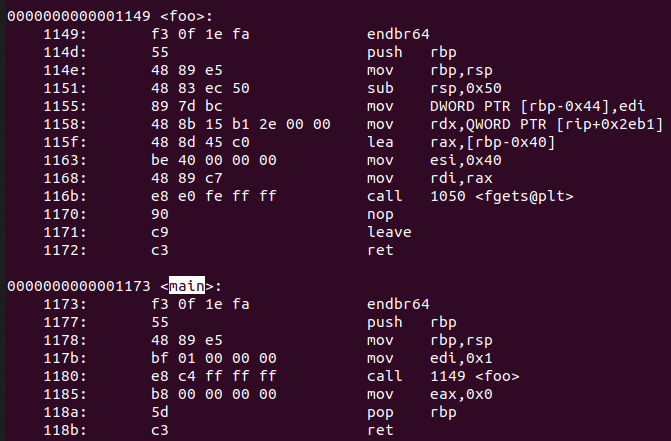
\includegraphics[width=\linewidth]{imgs/stack_overflow_counters/exe_without_canary.png}
\end{minipage}
\begin{minipage}[c]{0.473\linewidth}
    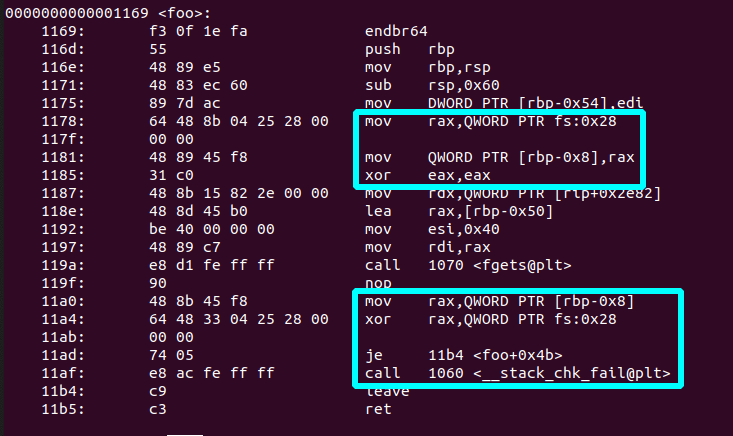
\includegraphics[width=\linewidth]{imgs/stack_overflow_counters/exe_with_canary.png}
\end{minipage}
    \caption{\texttt{foo} function without and with stack canary}
\end{figure}

Checking for a value every time a function returns comes with a performance penalty and for that reason compilers allow opting out from using stack canaries. Compilers usually compile with stack protectors by default. To compile a program without stack canaries in \texttt{gcc} use the \texttt{-fno-stack-protector} option. Some compilers have options to specify which functions you want to be compiled with stack canaries to achieve a trade-off between performance and security.

\begin{figure}[H]
\centering
    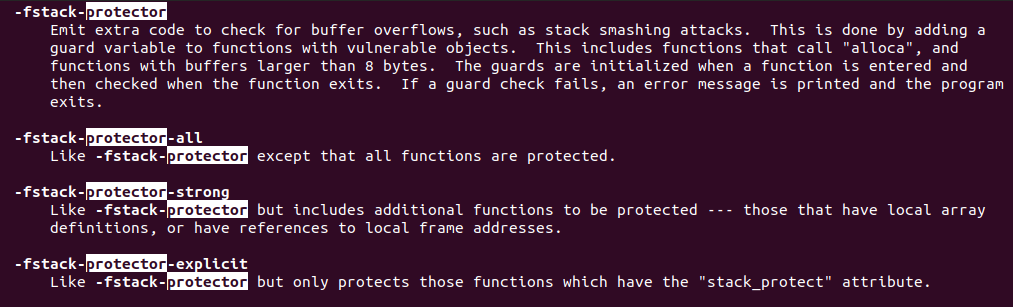
\includegraphics[width=\linewidth]{imgs/stack_overflow_counters/man_gcc_stack_protector}
    \caption{\texttt{man gcc}}
\end{figure}

\subsection{Check for canaries}
To check for the existence of canaries on a binary we can take a look at the disassembled code or we can search for the symbol \texttt{\_\_stack\_chk\_fail}\cite{checksec:github}, the function that checks the canary integrity.
\begin{lstlisting}[language=bash]
readelf -s a.out | grep -q '__stack_chk_fail'
\end{lstlisting}


\subsection{Bypassing stack canaries}
\subsubsection{Leaking the stack canary}
Stack canaries are not bulletproof though and can be bypassed. If you include the stack canary value in your input when you overflow the stack the canary checking function will not detect the stack overflow. Note that the canary value in the input must align with the canary value in the stack. So to bypass the canary we need to know its value, a value that changes every time the binary is executed. If we could make the binary reveal its contents in runtime we could read the canary value. We have to \textbf{leak} it (see subsection \ref{format_strings:arbitrary_read}).

\subsubsection{Bruteforcing the stack canary}
There is also a bruteforce approach to processes that use the \texttt{fork} function for POSIX systems. \texttt{fork} copies the hole process image from the parent to the child, stack canaries included. Therefore, the canaries are the same for both the child and the parent. This is useful for programs like web servers that use \texttt{fork} to handle the incoming connections. The bruteforce approach consist of leaking the canary one byte at the time.
\begin{lstlisting}[caption={Pseudocode for bruteforcing a canary in a \texttt{fork} program}]
uint8_t canary[STACK_CANARY_WIDTH];

for(int i = 0; i < STACK_CANARY_WIDTH; ++i)
{
    for(int j = 0; j < 256; ++j)
    {
        canary[i] = j;
        send(buffer + canary[:i+1]); /* only send the first i bytes of the canary */
        if(!fork_child_crashed)
            break;
    }
}
\end{lstlisting}
This algorithm reduces the entropy space from $256^{\texttt{STACK\_CANARY\_WIDTH}}$ to $256\times \texttt{STACK\_CANARY\_WIDTH}$.

\subsubsection{Bypass using Exception Handling}
Another technique to bypass stack canaries consist of triggering an exception before the canary is checked. If the attacker can overwrite an exception handler structure and trigger the exception a SEH based stack overflow exploit could be executed.\cite{corelan:bypass}
%https://0x00sec.org/t/exploit-mitigation-techniques-stack-canaries/5085
%https://www.exploit-db.com/docs/english/17505-structured-exception-handler-exploitation.pdf

\subsubsection{Replace the canary value}
Replace the authoritative canary value in the \texttt{.data} section of the program. Because the canary is computed at runtime the section where it resides must be marked as writable. To use this technique an arbitrary write is needed.

\subsubsection{Arbitrary writes}
An arbitrary write implies the ability to write an arbitrary value to an arbitrary memory location marked as writable. This means that we can write values on addresses that are not contiguous to our overflow, giving us the possibility to overwrite the return address without having to overwrite the stack canary.


\section{NX/DEP/W$\oplus$X}
\label{stack_overflow_countermeasures:NX}
\textbf{NX} is a protection that marks a memory region as non-executable. Different operating systems and architectures present different mechanism to implement the same concept. On Microsoft Windows it is called Data Execution Protection. On BSD systems it is called write $\oplus$ execute, refering to the rule that no memory section should be marked as writable and executable at the same time. The terms can, and they will, be used interchangeably.

On the previous exploit we returned to the stack where we loaded instructions. Now, if the stack is marked as non-executable, those instructions on the stack cannot be executed: the CPU will throw an exception.

\subsection{Check for NX}
To check for this security feature on a binary we can take a look at the permissions of the section where the stack will be loaded\cite{checksec:github}. Again, this depends on the compiler, the OS and the architecture.
\begin{lstlisting}[language=bash]
readelf -W -l a.out | grep 'GNU_STACK'
\end{lstlisting}

\section{ASLR/PIE}
\textbf{ASLR} is the acronym of Address Space Layout Randomization. It is a feature that randomizes the location of the libraries on the process memory, rendering useless attacks with hardcoded addresses, like our second exploit.

Every time an executable is launched, the OS needs to create the process memory space and the loader loads the dynamic libraries the process requires on certain addresses. Conventionally, those addresses were resolved at compile time and were included on the executable. The executable format contains indications for the OS on how to create its process and where it expects the libraries to be located. That caused that the addresses of the libraries where known and predictable.
To make them harder to exploit, the kernel randomizes the location of those libraries every time the executable is executed.\\

To compile a program without ASLR/PIE support on \texttt{gcc} use the \texttt{--no-PIE} option.

\subsection{Check for ASLR/PIE}
For ASLR to work, the operating system needs to support it \textbf{and} applications must be compiled with ASLR in mind. Because the load locations are unknown at compile time, the compiler needs to create a \textbf{Position Independent} Code or Executable.
To check if the OS has ASLR enabled:
\begin{lstlisting}[language=bash]
cat /proc/sys/kernel/randomize_va_space
# 0 = Disabled
# 1 = Conservative randomization
# 2 = Full randomization
\end{lstlisting}
To check if a binary has been compiled with ASLR support\cite{checksec:github}:
\begin{lstlisting}[language=bash]
readelf -h a.out | grep "DYN"
\end{lstlisting}

% https://reverseengineering.stackexchange.com/questions/6657/why-does-ldd-and-gdb-info-sharedlibrary-show-a-different-library-base-addr
Additionally, in Linux systems we can use the \texttt{LD\_TRACE\_LOADED\_OBJECTS} environment variable to modify the behavior of the loader, which prints out the dynamic library dependencies and their addresses where they were loaded at runtime. In systems with ASLR enabled, those addresses will be different each time the same command is executed. In systems where ASLR is disabled, the addresses will always be the same.

\begin{figure}[H]
\begin{minipage}[c]{0.5\linewidth}
    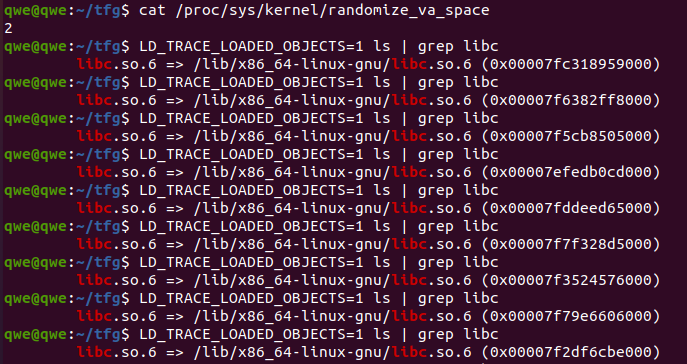
\includegraphics[width=\linewidth]{imgs/stack_overflow_counters/addresses_aslr.png}
\end{minipage}
\begin{minipage}[c]{0.5\linewidth}
    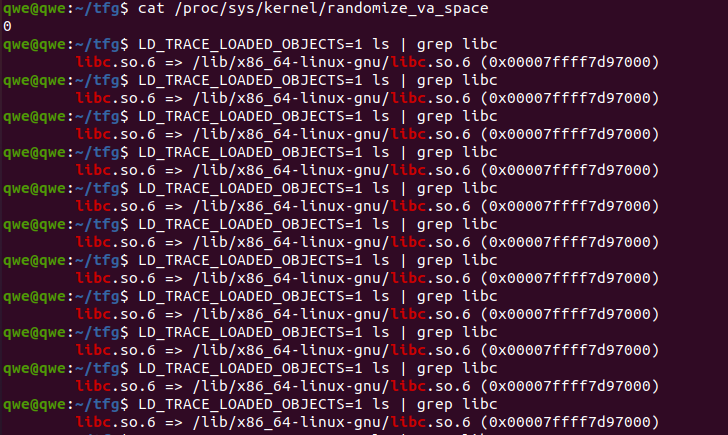
\includegraphics[width=\linewidth]{imgs/stack_overflow_counters/addresses_without_aslr.png}
\end{minipage}
    \caption{libc base address loaded at runtime with ASLR enabled/disabled}
\end{figure}

\end{document}

